\documentclass[a4paper, 11pt, oneside]{article}

\newcommand{\plogo}{\fbox{$\mathcal{PL}$}} 
\usepackage{amsmath}
\usepackage[utf8]{inputenc} 
\usepackage[T1]{fontenc} 
\usepackage{enumitem}
\usepackage{graphicx}
\usepackage{graphicx}
\usepackage{supertabular}
\usepackage[spanish]{babel}
\usepackage{hyperref}
\graphicspath{{Imagenes/}}

\begin{document} 

\begin{titlepage} 

	\centering 
	
	\scshape 
	
	\vspace*{\baselineskip} 
	
	
	
	\rule{\textwidth}{1.6pt}\vspace*{-\baselineskip}\vspace*{2pt} 
	\rule{\textwidth}{0.4pt} 
	
	\vspace{0.75\baselineskip} 
	
	{\LARGE Practica 9: CentOS}	
	\vspace{0.75\baselineskip} 
	
	\rule{\textwidth}{0.4pt}\vspace*{-\baselineskip}\vspace{3.2pt}
	\rule{\textwidth}{1.6pt} 
	
	\vspace{2\baselineskip} 
	

	ADMINISTRACIÓN DE SISTEMAS UNIX/LINUX
	
	\vspace*{3\baselineskip} 
	
	
	
	Alumnos:
	
	\vspace{0.5\baselineskip} 
	
	{\scshape\Large Karla Adriana Esquivel Guzmán url{https://github.com/karlycaramelo} \\
    Eric Giovanni Miguel Torres url{https://github.com/EricGiovanni}\\ 
    María Ximena Lezama Hernández url{https://github.com/LezamaXi}\\ 
    Gonzalo Vazquez Cruz url{https://github.com/truerandom}}
	\vspace{0.5\baselineskip} 
	\vfill
	
\includegraphics[scale=0.65]{unam.jpg}
	
	\textit{UNIVERSIDAD NACIONAL AUTONOMA DE MEXICO} 
	
	\vfill
	
	
	
	
	\vspace{0.3\baselineskip} 
	
    30/Abril/2019 
	
	 

\end{titlepage}
\section*{Introducciión}
Ésta practica consiste en probar varias configuraciones de Display de VirtualBox con el Sistema Operativo CentOS.

\section*{Reporte}
\begin{itemize}
    \item Durante la instalación de CentOS tiene que configurarse la RED y activar la conexión vía Ethernet, o al concluir la instalación, el sistema operativo no va a tener funciones de Red.
    \begin{center}
        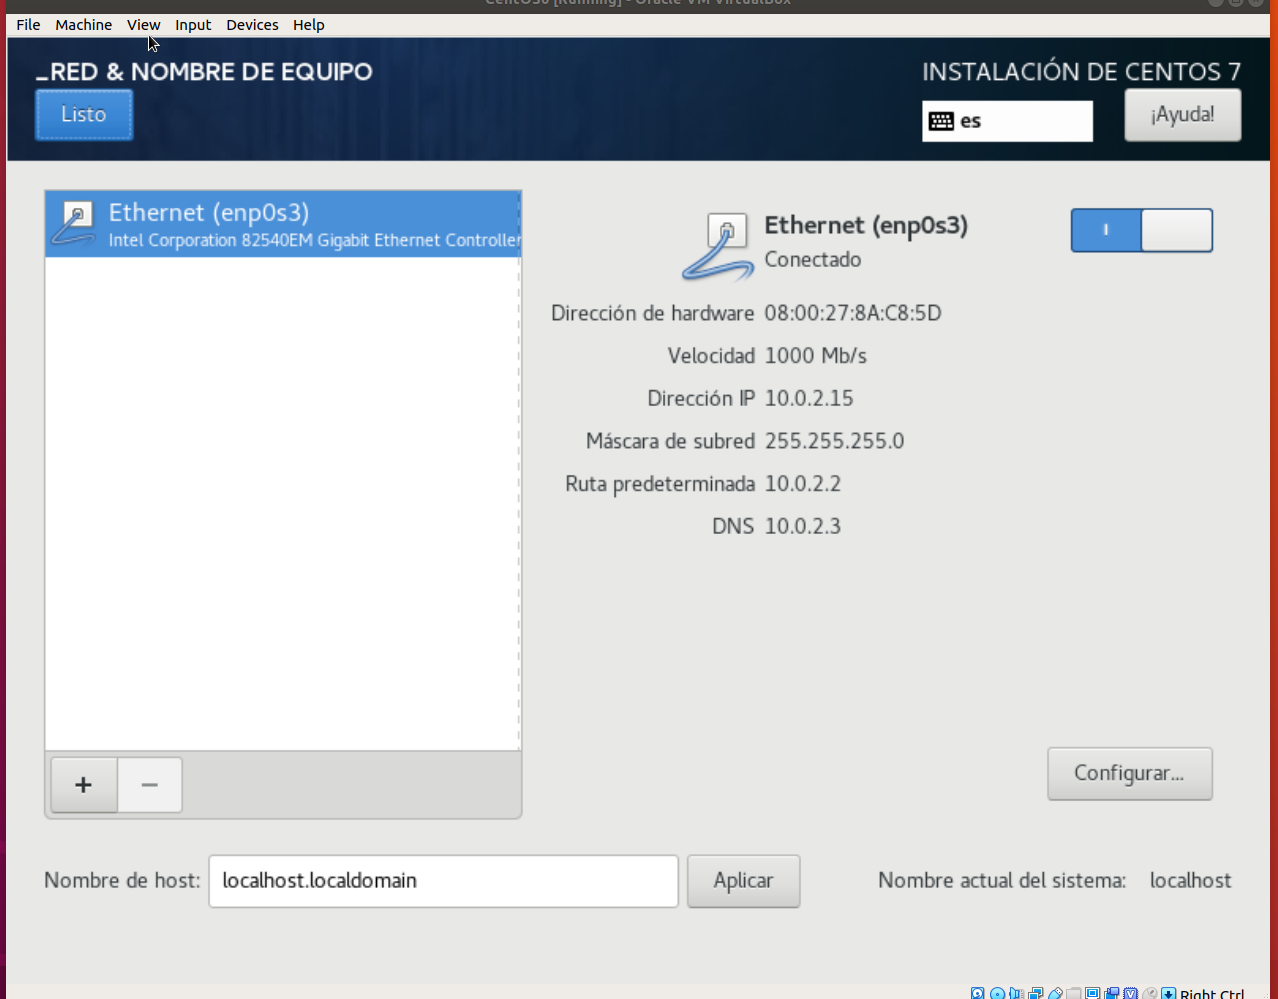
\includegraphics[scale=0.25]{ethernet.png}
    \end{center}
    \item Utilizamos Varias resoluciones entre ellas:
        \begin{itemize}
            \item 1024x768      (ésta fue la que más nos gustó) 
            \item 1600x1200     
            \item 1440x1050       
            \item 1280x960        
            \item 800x600         
            \item 640x480         

        \end{itemize}
        Experimentamos utilizando distintas configuraciones directamente cambiando los valores en 
        la sección "Display" de VirtualBox, incluído el controlador gráfico.
        
        \begin{center}
            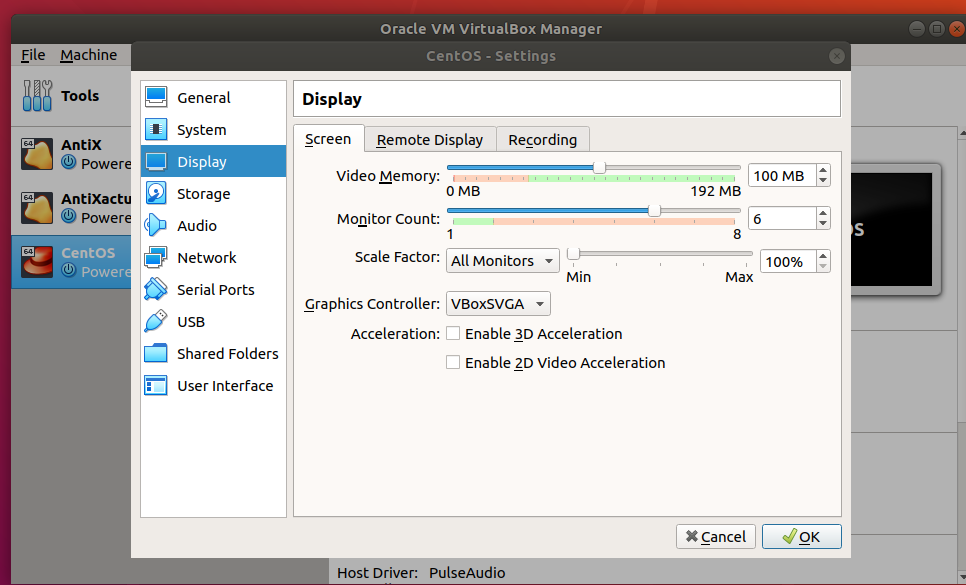
\includegraphics[scale=0.30]{display1.png}
        \end{center}
    \item Sin embargo también utilizamos los drivers que nos proporciona VirtualBox para distribuciones basadas en RedHat, para ello tuvimos que instalara en CentOS \textbf{VirtualBox Gust Addition}, como CentOS tiene problemas en VirtualBox con la integración del Mouse, instalar estos drivers nos ayudaron a solucionarlo, además proporciona el rendimiento de video acelerado.
    
    La instalación es muy sencilla simplemente se hace lo siguiente:
    \begin{enumerate}
        \item Se debe montar el dispositivo "VirtualBox Guest Additions"
        Esto se hace con mkdir /media/VirtualBoxGuestAdditions y mount -r /dev/cdrom /media/VirtualBoxGuestAdditions
        
        \item Después ocupamos el gestor de paquetes rpm para instalar los paquetes necesarios\\
        rpm -Uvh https://dl.fedoraproject.org/pub/epel/epel-release-latest-7.noarch.rpm
        
        \item Agregamos la variable de entorno :\\ KERN\_DIR=/usr/src/kernels/3.10.0-957.12.1.el7-x86\_64/build
        \item Por último ya podemos instalar Guest Additions con los siguientes comandos
        cd /media/VirtualBoxGuestAdditions y ./VBoxLinuxAdditions.run

    \end{enumerate}
    
    \begin{center}
        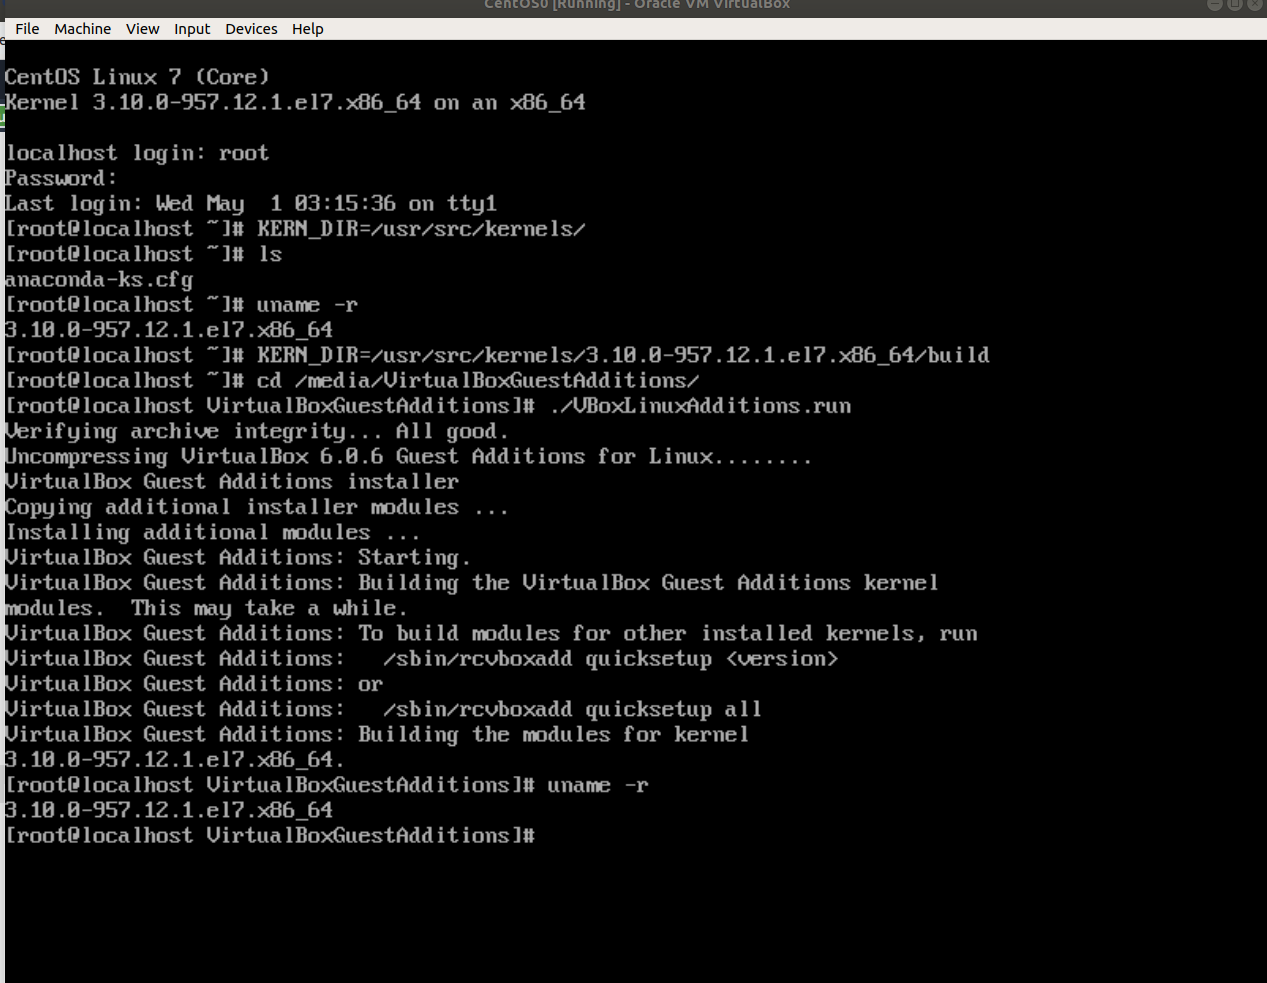
\includegraphics[scale=0.27]{additions.png}
    \end{center}
    
    Fuera de lo ya mencionado no tuvimos ningún otro inconveniente para manipular la resolución de la maquina virtual pues es muy sencillo cambiarlo manualmente desde la sección de configuración de virtualBox.
\end{itemize}
\end{document}